% Use only LaTeX2e, calling the article.cls class and 12-point type.

\documentclass[12pt]{article}

% Users of the {thebibliography} environment or BibTeX should use the
% scicite.sty package, downloadable from *Science* at
% www.sciencemag.org/about/authors/prep/TeX_help/ .
% This package should properly format in-text
% reference calls and reference-list numbers.

%\usepackage{scicite}
\usepackage{multirow}
\usepackage{graphicx}
\usepackage{amsmath,array,mathtools}
\usepackage{color,soul}
\usepackage[toc,page]{appendix}
\usepackage[symbol]{footmisc}

% Use times if you have the font installed; otherwise, comment out the
% following line.

\usepackage{times}

% The preamble here sets up a lot of new/revised commands and
% environments.  It's annoying, but please do *not* try to strip these
% out into a separate .sty file (which could lead to the loss of some
% information when we convert the file to other formats).  Instead, keep
% them in the preamble of your main LaTeX source file.


% The following parameters seem to provide a reasonable page setup.

\topmargin 0.0cm
\oddsidemargin 0.2cm
\textwidth 16cm 
\textheight 21cm
\footskip 1.0cm


%The next command sets up an environment for the abstract to your paper.

\newenvironment{sciabstract}{%
\begin{quote} \bf}
{\end{quote}}


% If your reference list includes text notes as well as references,
% include the following line; otherwise, comment it out.

\renewcommand\refname{References and Notes}

% The following lines set up an environment for the last note in the
% reference list, which commonly includes acknowledgments of funding,
% help, etc.  It's intended for users of BibTeX or the {thebibliography}
% environment.  Users who are hand-coding their references at the end
% using a list environment such as {enumerate} can simply add another
% item at the end, and it will be numbered automatically.

\newcounter{lastnote}
\newenvironment{scilastnote}{%
\setcounter{lastnote}{\value{enumiv}}%
\addtocounter{lastnote}{+1}%
\begin{list}%
{\arabic{lastnote}.}
{\setlength{\leftmargin}{.22in}}
{\setlength{\labelsep}{.5em}}}
{\end{list}}


% Include your paper's title here

\title{Energy and Time Determine Scaling in \\Biological and Computer Designs} 
%Biological and Computer Designs Minimize Energy and Time.  

% Place the author information here.  Please hand-code the contact
% information and notecalls; do *not* use \footnote commands.  Let the
% author contact information appear immediately below the author names
% as shown.  We would also prefer that you don't change the type-size
% settings shown here.

\author
{Melanie Moses,$^{1,2,3\ast}$ Stephanie Forrest$^{1,2,3}$ George Bezerra,$^{1}$ \\Benjamin Edwards$^{1}$, James Brown,$^{2,3}$ \\
\\
\normalsize{$^{1}$Department of Computer Science}\\
\normalsize{University of New Mexico, Albuquerque, NM, USA.}\\
\normalsize{$^{2}$Department of Biology}\\
\normalsize{The University of New Mexico, Albuquerque, NM, USA.}\\
\\
\normalsize{$^{3}$The Santa Fe Institute, Santa Fe, NM, USA.}\\
\\
\normalsize{$^\ast$To whom correspondence should be addressed}\\
\normalsize{E-mail: melaniem@cs.unm.edu}\\
\normalsize{Address: Department of Computer Science}\\
\normalsize{1 University of New Mexico, Albuquerque, NM USA}\\
\normalsize{Phone: 505-277-3112}\\
}



% Include the date command, but leave its argument blank.

\date{\normalsize{{\bf Keywords:} network scaling, power consumption, 
metabolic rate, complex systems, energy-time product, organism, 
computer chip}\\
\normalsize{{\bf Classification:} Major: ; Minor: }}



%%%%%%%%%%%%%%%%% END OF PREAMBLE %%%%%%%%%%%%%%%%



\begin{document} 

\newcounter{casenum}
\newenvironment{caseof}{\setcounter{casenum}{1}}{\vskip.5\baselineskip}
\newcommand{\case}[2]{\vskip.5\baselineskip\par\noindent {\bfseries Case
\arabic{casenum}:} #1: #2\addtocounter{casenum}{1}}

% Double-space the manuscript.

\baselineskip24pt

% Make the title.

\maketitle 


\newpage

% Place your abstract within the special {sciabstract} environment.
% \centerline{\Large{\bf Abstract}}
% \begin{sciabstract}
% Metabolic rate in organisms and power consumption in computers are 
% analogous quantities that scale similarly with size.  We analyze 
% organisms and computer chips as systems in which natural selection or 
% human engineering has produced optimized networks that minimize the 
% energy-time product.  The network designs simultaneously reduce energy 
% costs and increase flow rates.  Using a simple network model, our 
% analysis explains empirically observed trends in the scaling of 
% metabolic rate in organisms and power consumption in chips across 
% several orders of magnitude in size.  This result suggests that a 
% single principle governs the designs of many complex systems that 
% process energy, materials, and information.
% \end{sciabstract}

% Place your abstract within the special {sciabstract} environment.
% The new abstract
\centerline{\Large{\bf Abstract}}
\begin{sciabstract}
  Metabolic rate in animals and power consumption in computers are
  analogous quantities that scale similarly with size.  We analyze
  vascular systems of vertebrates and on-chip networks of
  microprocessors, where natural selection and human engineering
  respectively have produced optimized networks.  
% 'modeled  here as the energy-time product'?
Both network designs
  simultaneously reduce energy costs and increase flow rates.  Using a
  simple network model, our analysis explains empirically observed
  trends in the scaling of metabolic rate in organisms and power
  consumption in chips across several orders of magnitude in size.
  This result suggests that a single principle governs the designs of
  complex systems that process energy, materials, and
  information. Just as fundamental shifts in metabolic energy have accompanied the evolutionary transitions in biology, our models suggest that energy efficiency will change as computer technology becomes more distributed and decentralized in the shift to multi-core and dispersed cyber-physical systems. Scaling 
  
  
\end{sciabstract}

\newpage

\section{Introduction}
\label{sec:intro}

Both organisms and computers have evolved from relatively simple beginnings
into complex systems that vary by orders of magnitude in size and number of
components. Evolution, by natural selection in organisms and by human
engineering in computers, required critical features of architecture and
function to be scaled up as size and complexity increased. In Biology,
Kleiber's law describes the empirical relation between metabolic rate and many
other traits, such as lifespan, heart rate, and number of offspring, with body
size \cite{kleiber47}.  Similarly, computer architecture has Moore's law to
describe scaling of transistor density and performance \cite{moore98}, Koomey's
law for the energy cost per computation \cite{koomey11}, and Rent's rule for
the external communication per logic block \cite{christie00}.

% We posit that these empirical patterns originate from a common 
% principle: Networks that deliver resources are optimized to reduce 
% energy dissipation and increase flow rates, expressed here as 
% minimizing the energy-time product. {\bf Need to clarify where energy
%   is disipated.  we ention energy-time product but rest of paragraph
%   is about the network and not the nodes.}  In biology, the vascular network 
% of vertebrate animals supplies oxygen and nutrients to every cell, 
% fueling metabolism for maintenance, growth and reproduction.  Since 
% energy is a limited resource, organisms are selected to minimize the 
% energy dissipated in the network \cite{west97}. Similarly, computation 
% in microprocessors relies on a network of microscopic wires that 
% transmits bits of information between transistors on a chip.  In order 
% to maximize computer performance and minimize power consumption, this 
% network is designed to deliver the maximum information flow at the 
% lowest possible energy cost.

We posit that these empirical patterns originate from a common principle:
Networks that deliver resources are optimized to reduce energy dissipation and
increase flow rates, expressed here as minimizing the energy-time product. That
is, both living systems and computer chips are designed to maximize the rate at
which resources are delivered to terminal nodes of a network and to minimize
the energy cost in the network.  In biology, the vascular network of vertebrate
animals supplies oxygen and nutrients to every cell, fueling metabolism for
maintenance, growth and reproduction.  Since energy is a limited resource, we
assume that organisms are selected to minimize the energy dissipated in the
network \cite{west97}. Similarly, computation in microprocessors relies on a
network of microscopic wires that transmits bits of information between
transistors on a chip.  In order to maximize computation speed and minimize
power consumption, this network is designed to deliver the maximum information
flow at the lowest possible energy cost.

Here, we model vertebrates as composed of regions of tissue that receive oxygen
carried by blood via a hierarchical vascular network of pipes, and we model
microprocessors as composed of transistors that perform computation, exchanging
information over a modular network of wires.  As each system scales up in size,
we consider: 1) the rate at which resources are delivered by the network and
processed in the nodes; and 2) the energy dissipated during these processes.
Despite the obvious differences between organisms and chips, we present a
general model and derive energy and time scaling relations from physical
principles applicable to each system. Using these relations, we express the
optimal network design as a tradeoff between energy cost and processing speed. 

% Here, we model vertebrates as composed of regions of tissue that 
% receive blood via a hierarchical vascular network of pipes, and we 
% model microprocessors as composed of transistors that perform 
% computation, exchanging information over a modular network of wires.  
% As each system scales up in size, we consider: 1) the time for 
% resources to flow through the network and be processed in the nodes; 
% and 2) the energy dissipated during these processes. Despite the 
% obvious differences between organisms and chips, we derive general 
% energy and time scaling relations from physical principles applicable 
% to each system. Using these relations, we express the optimal network 
% design as an energy-time product minimization problem.

Earlier models in biology have assumed either energy minimization, e.g.,
\cite{west97} or optimal resource delivery rate \cite{banavar10}, but they have
not formalized the tradeoffs between them, as we do here.  This formalization
helps explain how  nature and engineering are able to produce designs that
approach pareto-optimal along the energy-time tradeoff.  Thus, in biology
evolution has produced mammals ranging in size from mice to elephants, rather
than converging on a single optimal size, and in computer architecture
engineers have designed processors ranging from a few thousand transistors to
several billion, each of which fills a specific computational niche.

In the rest of the paper, we first present the unified model of network
scaling (Section \ref{sec:unified-model}) and the basic assumptions underlying
the model (Section ~\ref{sec:assumptions}).  We then use the model to derive a series of predictions about how time and energy scale with system size first for 
organisms (Section \ref{sec:organisms}) and then for computers (Section
\ref{sec:computers}). We then discuss new insights into previously analyzed scaling relationships in biology that we gain from the time-energy minimization framework, and we test scaling predictions with empirical power and performance data on computer chips.  Finally, in Section
  \ref{sec:discussion}  we discuss
  the implications of these results for evolutionary transitions in
  nature and engineering.

\begin{figure}[!h]
\centering
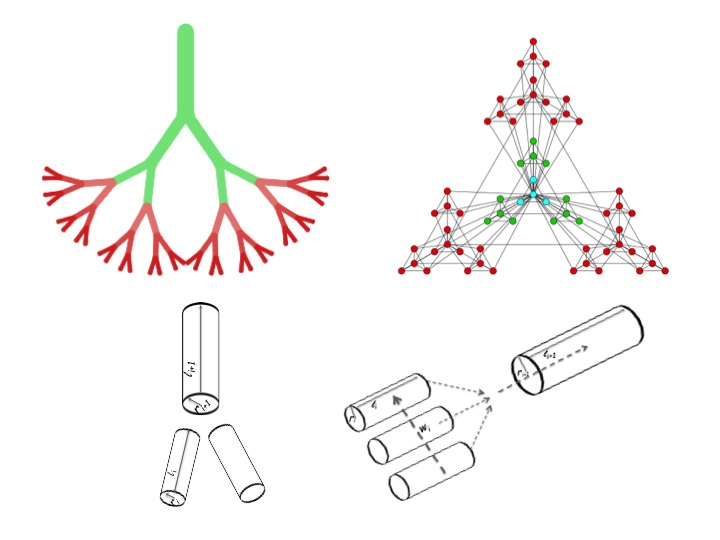
\includegraphics[height=90mm]{Figures/Figure1Draft.jpg}
\label{fig:firstfig}
\caption{Panel a: idealized fractal branching model of the cardiovascular network. Explain Dl, Dr, lambda H N and slowing by referring to the picture. 
Panel c illustrates the communication dimension, $D_w$,
  which measures how the ratio of internal (intra-module) communication per node to
  external (inter-module) communication per node scales with the level of the module in
  the hierarchy. Keep b and d? }
\end{figure}
\section{A Unified Model of Network Scaling}
\label{sec:unified-model}


Vascular systems are hierarchical branching networks where blood vessels
(pipes) become thicker and longer as hierarchy increases from the capillaries
to the aorta. Similarly, microprocessor chips are organized hierarchically into
a nested structure of modules and submodules, where wires become longer and
thicker as the hierarchical level of a module increases
(Figure~\ref{fig:firstfig}).  These wires are organized into metal
layers, where short, thin wires are routed on the lowest layers, and long,
thick wires are placed on the top layers. We model the scaling of length ($l$)
and thickness ($r$) of both pipes and wires as

\begin{equation}
l_i = l_0 \lambda^{\frac{i}{D_l}}
\end{equation}

\noindent and

\begin{equation}
  r_i = r_0 \lambda^{\frac{i}{D_r}},
\label{eq:rscaling}
\end{equation}

\noindent where $i$ is the hierarchical level of a branch or module, $\lambda$
is the branching factor, and $D_l$ and $D_r$ are the length and thickness
dimensions. This model is akin to the hierarchical pipe model of vascular
systems proposed in \cite{west97}, $\lambda^{\frac{1}{Dr}}$ and
$\lambda^{\frac{1}{Dl}}$ correspond to West et al.'s $\beta$ and $\gamma$
respectively (note that in~\cite{west97}, the aorta or top of the network is labelled as level 0,
while here the smallest branches, the capillaries, are labelled as level 0.)
% where $l_i$ ROUGHLY corresponds to $\gamma$
%and $r_i$ ROUGHLY corresponds to $\beta$.  
In vascular networks, $r$ represents the radius of cylindrical pipes, and in
computer interconnects, $r$ represents the width of wires with aspect ratio 1.  $D_r$ describes the relative radius of pipes between successive hierarchical levels. 
The smallest edges occur at $i = 0$, and have constant radius,
$r_0$, and length, $l_0$, that scales with system size~\cite{banavar10}. 

%\begin{figure}
%\caption{Schematic: Panel c illustrates the communication dimension, $D_w$,
%  which measures how the ratio of internal (intra-module) communication per node to
%  external (inter-module) communication per node scales with the level of the module in
%  the hierarchy. Note, that if we had a biological version, we would
%  have MORE edges.}
%  \label{fig:model-schematic}
%\end{figure}

The length parameter $D_l$ determines the spatial dimension occupied by the
nodes of the network \cite{mandelbrot83}.
For chips, $D_l = 2$, since transistors are placed on a single
two-dimensional layer \cite{donath81}. For three-dimensional organisms,  $D_l = 3$. $D_l$ describes both the relative length of pipe between successive hierarchical levels and the external dimension of the system.

Digital circuits scale in a third way in addition to length and radius, which
has no direct analog in organisms. In vascular networks, each pipe 
branches at each hierarchical level (generally bifurcating so that $\lambda = 2$~\cite{SavageCompBio2015}.) Chips have multiple wires per module, and their number
increases with the hierarchical level. This difference arises from the fact
that digital circuits are decentralized networks connecting multiple sources
and destinations, while vascular networks are centralized, with blood flowing
from a single heart. To account for this difference, we introduce a new
equation, in which the communication (or number of wires) per module increases
with the hierarchical level as

\begin{equation}
w_i = w_0 \lambda^{i/D_w},
\label{eq:communication}
\end{equation}

\noindent where $D_w$ is the communication dimension and $w_0$ is the average
number of wires per node.  This hierarchical scaling of communication is a
well-known pattern in circuit design called Rent's rule \cite{christie00},
where $p = \frac{1}{D_w}$ is the Rent's exponent.\footnote{Rent's rule is typically
  expressed as $C(n) = kn^p$, where $C_n$ is the external communication of a
  module, $n$ is the size of the module (number of nodes), $k$ is the average
  external communication of a module with size 1, and $p$ is the Rent’s
  exponent. For a hierarchy with branching factor of $\lambda$, the size of a
  module is given as $n = \lambda^i$, where $i$ is the hierarchical level.
  Therefore, we can rewrite Rent’s rule as $c_i = c_0 \times \lambda^{ip}$,
where $c_0 = w_0$ and $p = \frac{1}{D_w}$.} This pattern is not unique to circuits
and has been shown to occur in many biological networks
\cite{reda09,bassett10}.   Vascular systems correspond to a special case where 
%$w_0 = 1$ and $1/D_w = 0$, such that 
$w_i = 1$ for all $i$. 

\subsection{Assumptions of the Unified Model}
\label{sec:assumptions}

Before deriving scaling predictions from the model, we make explicit
its  assumptions and how they relate to earlier models, both in
computation and biology:

\begin{enumerate}
\item {\bf Time and energy are equally important constraints:} 
  System designs seek to deliver the maximum amount of
  resource per unit time for the minimum amount of energy overhead. 
%interpreted as minimizing the energy dissipated to deliver
%  and process a unit of resource, while simultaneously minimizing the
%  time to deliver and process that resource.  
  In computer architecture this relationship is expressed as the
  \emph{energy-delay product}, which formalizes the insight that a
  chip that is ten times faster or ten times more energy efficient is
  ten times better. 
%It is
%unrealistic that either of these quantities is minimized independently
%of the other.
%WHY ISN'T IT ADDITIVE?
% A multiplicative decrease of either quantity should be reflected
% proportionally by the energy-delay equation.  i.e., a chip that is
% 10 times faster, should make the energy-delay equation 10 times
% better.  Has something to do with multiplicity of components.

\item {\bf Steady state}: Resource supply matches processing
  demand~\cite{banavar10}.  That is, the network supplies resources continually
  to the terminal nodes and is always filled to capacity.  This avoids network
  delays and the need to store resources in the system. Specifically,

  \begin{enumerate}

\item System designs balance network delivery rates with node processing
  speeds, so that resources are delivered at exactly the same rate that they
  are processed.

\item Pipelining: A concept from computer architecture in which resources,
  e.g., computer instructions, leave the source at the same rate that they are
  delivered to the terminal nodes, and the network is always full.  In the
  hierarchical networks considered here, the source is the highest branch
  (root), and the principle holds within every level of the hierarchy.
  Consequently, resources flow through the network continually at maximum
  speed, and they do not accumulate at source, sink, or intermediate locations.
  \end{enumerate}

\item {\bf Terminal units and service volumes:} In contrast to
  Ref.~\cite{west97} we do not assume that terminal units have fixed size.   In
  chips it is well known that transistor size has shrunk over many orders of
  magnitude.   Previous scaling models of biology posit that the service volume
  (region served by terminal units of the network) actually increases with
  system size~\cite{west97,banavar10}.  Following Ref.~\cite{banavar10}, we
  assume that capillaries have fixed radius but that their length is
  proportional to the radius of the service volume.   Similarly, the radius of
  the isochronic region (service volume) for chips scales proportionally with
  decreasing transistor size.
% really we mean 'length' of one side of the transistor, aka process size.
\end{enumerate}

In addition to these general assumptions, we make the following
refinements to accommodate salient differences between biology and computer architecture.
\begin{enumerate}
\item In biology, the energy processed by a service volume,
  $E_{node}$, is invariant with system size. That is, as the service volume
  increases with body size, the total amount of energy processed
  remains constant.   We do not make this assumption for chips.

\item Component packing: In chips, we assume that total chip area is constant, and the
  number of transistors $N$ is the square of the process size, i.e.,
  the length of one side of a transistor. 

\end{enumerate}

\noindent 

In biology it is known that blood flow slows by several orders of magnitude as it travels from the aorta to the capillaries (CITE somebody). Scaling models have generally ignored this slowing~\cite{west97, banavar10}, but we leave this variable in our equations to highlight where velocity affects time and energy scaling.

\section{Predictions of the Model for Organisms and Computers}
%\label{sec:}

We define $E_{net}$ and $T_{net}$ respectively to be the energy dissipated and
the time taken by the network to deliver a unit of resource to each node.  For
organisms the resource is oxygen (in mammals, carried by a unit volume of
blood), and for computers the fundamental resource is a bit of information.
Similarly, we define $E_{node}$ and $T_{node}$ as the energy dissipated and the
time taken by the nodes to process that resource.  For organisms, the node is the
service volume corresponding to a region of tissue supplied by a single
capillary, which corresponds to a volume of tissue containing a constant number of mitochondria, the organelles that process
oxygen molecules to generate biologically useful energy in the form of ATP. %(Citations needed: banavar? Jordan's paper, maybe Woodruff paper?)
The node is defined as having a constant rate of delivery of oxygen and a constant ability to process oxygen, but the volume of the nodes vary across organism size. 

$E_{net}$ is the energy required to deliver oxygen to the cells (as
analyzed in \cite{west97}), and $E_{node}$ is the energy dissipated by cells
processing incoming oxygen. $T_{net}$ and
$T_{node}$ are the time delay between delivering new resources to the cell and
the time taken for the cell to process those resources respectively. From the
steady-state assumption, $T_{net} = T_{node}$, i.e., supply matches demand as in ~\cite{banavar10}.

For computers, the nodes are transistors, and 
%$E_{net}$ and $T_{net}$ correspond to the energy dissipated and the time taken
%to transport a bit of information to a node over the network, and 
$E_{net}$ and $E_{node}$ represent the energy dissipated as bits are delivered to
transistors and the energy required to process the bits at the node, and
$T_{net}$ and $T_{node}$ are the times required to deliver and process a bit at
the node (i.e., network and transistor switching delay).  In computers the time
taken to deliver and process bits is bounded by the maximum of the
communication time $\max(T_{net},T_{node})$, i.e. a node cannot process
another bit until it is delivered, and a node cannot process a new bit until it
is done processing the previous bit. %Because of the steady state assumption $T_{net}$ and $T_{node}$ are equal. 
In contrast to Biology, as we show below, the network delivery rate does not match the uptake rate at the nodes.  Thus,  for biology the total delay is defined as
$T_{sys}=T_{net} = T_{node}$ while for computers the total delay is defined as
$T_{sys}=\max(T_{net},T_{node})$. For both organisms and computers we define
the total energy as the sum of energy dissipated in the network plus the energy dissipated in the nodes: $E_{sys} = E_{net} + E_{node}$.

%Note, the service volume is not necessarily of fixed size~\cite{banavar10}.
 In the following, we derive general 
scaling relationships between $E_{net}$, $T_{net}$, $E_{node}$ and $T_{node}$ and the number of nodes in the network $N$, under the condition that the energy time product is minimized.  $N$ is a measure of system size (i.e. the number of capillaries or services volumes in an organism and the number of transistors on a chip). In organisms, larger $N$ implies larger organism volume and mass. For computer chips, $N$ increases by shrinking components, and so increasing $N$ does not imply increasing chip area, which we assume to be constant.

 The goal of minimizing the energy time product means that system designs seek to deliver the maximum amount of
resource per unit time for the minimum amount of energy overhead.   This is
equivalent to minimizing the energy dissipated to deliver and process a unit of
resource, while simultaneously minimizing the time to deliver and process that
resource.  Assuming that time and energy are equally important, this quantity
becomes the energy-time product, a well-known concept in computer architecture
referred to as the energy-delay product.  

%For computers, the nodes are isochronic regions (the service area supplied by a
%single clock signal),
%%We hypothesize that both organisms and computers maximize performance and minimize cost through
%scaled designs, where performance is given by resource flow (the rate at which a resource is delivered to and processed by the node), and cost is given by energy
%dissipated in the network and by the nodes, normalized per unit of resource processed.

%The hypothesis that organisms and computers minimize the energy-time 
%product predicts that scaled designs lie in a critical region of the 
%design space with the highest performance per cost, where performance 
%is given by flow and cost by energy.  
%To show this mathematically, we 
%use the general scaling relations from Table \ref{tab:equations} and 
We express the optimal network design as a constraint optimization 
problem in which the whole system's energy-time product is minimized:

\begin{equation}
  \min_{D_r,D_w,D_l}(E_{sys} \times T_{sys})
\label{eq:TheWholeEnchilada}
\end{equation}

%\noindent where the system's energy is given as $E_{sys} = E_{net} + E_{node}$,
%and the system's time as $T_{sys} = \max(T_{net}, T_{node})$.

We derive expressions for $E_{sys}$ and $T_{sys}$ for organisms
(Sec.~\ref{sec:organisms}) and computers (Sec.~\ref{sec:computers}) in
terms of the dimensions $D_r$, $D_w$, and $D_l$ where $D_l$ is fixed by the external dimensions of the system.

%The resulting scaling equations are summarized in Table \ref{tab:equations}.

% \begin{table}[!h]
% \caption{General energy and time scaling relations for organisms and 
% computers.  The relations are written as a function of the number of 
% nodes ($N$), which is a proxy for size, and the length and thickness 
% dimensions ($D_l$ and $D_r$), which determine network geometry. $c$ is a constant}

% \label{tab:equations}
% \centering
% \def\arraystretch{1.7}
% \begin{tabular}{|c|c|c|c||c|c|c|}\hline
%  & $E_{net} $ & $E_{node}$ & $E_{sys}$ & $T_{net}  $ & $T_{node}$ & $T_{sys}$\\ \hline

% Organism & $\propto N^{\frac{2}{D_r}-1}$ & $\propto N^0 \propto c$ &  $\propto N^{\frac{2}{D_r}-1} + c$ &
% $\propto N^{1 - \frac{2}{D_r}}$  & $\propto N^{1 - \frac{2}{D_r}}$ & $\propto N^{1 - \frac{2}{D_r}}$ \\ \hline

% Computer & $\propto N^{-\frac{1}{D_w}}$ & $\propto N^{-\frac{1}{D_l}}$ & $\propto N^{-\frac{1}{D_l}}$ & $\propto N^0$ & $\propto N^{-\frac{1}{D_l}}$ & $\propto N^0 + N^{\frac{1}{D_l}}$\\ \hline
% %Computer & $\propto N^{-\frac{1}{D_w}}$ & $\propto N^{-\frac{1}{D_l}} & $\propto N^{-\frac{1}{D_l}}$ & $\propto N^0$ & $\propto N^{-\frac{1}{D_l}}$  TSYS &  \\ \hline

% \end{tabular}
% \end{table}

\subsection{Organisms}
\label{sec:organisms}

In this section, we derive general energy and time scaling relations 
for the network and nodes in organisms in order to minimize Eq. \ref{eq:TheWholeEnchilada}.  
We first define scaling relationships for the four key quantities $E_{net}$, $T_{net}$, $E_{node}$ and $T_{node}$. We then show how they scale with $N$, in order to minimize Eq. 4. In contrast to computer scaling, biological scaling relationships have been examined in many different theoretical models (CITE lots of theoretical models). Two of those models ~\cite{west97, banavar10}  determined scaling relationships by separately minimizing energy dissipation ~\cite{west97} and minimizing metabolic delivery time ~\cite{banavar10} . Here we emphasize the consequences of incorporating these approaches into the broader computational scaling framework of minimizing the energy time product. 

$E_{net}$: From basic principles of hydraulics, the energy dissipated to
transport a constant volume of blood through the network
is given by the loss in pressure from the aorta to the capillaries
multiplied by the volume being transported.  Pressure is the product between
hydraulic resistance ($R$) and flow ($Q$), so the loss in pressure $\Delta P = RQ$.  Thus $E_{net}
\propto \Delta P \propto RQ$. 


$E_{node}$: Following ~\cite{west97} and (CITE mosesamnat08) we assume that the quantity of energy dissipated to metabolize a fixed quantity of oxygen in each node is constant so that the, energy summed over all nodes is
$E_{node} \propto N$.


$T_{net}$: The time to deliver a fixed number of oxygen molecules to the nodes is given by the volume of blood being transported divided by the flow ($Q$).  Since a constant volume is delivered to each node in parallel, we consider the volume being distributed per unit time to all nodes, giving $T_{net}\propto N/Q$.  

We note that there is no distance term in the $T_{net}$ equation because of the steady-state assumption. $T_{net}$ is the time it
takes to deliver the `next' oxygen molecule from a capillary. Thus $T_{net}$ is not the time it
takes a single molecule to traverse the network (i.e. it is not $\tau$ in~\cite{banavar10}, but rather the inverse of the rate of of delivery of oxygen molecules, analogous to the inverse of clock speed in computer chips.




$T_{node}$: Following \cite{banavar10} and under the steady-state assumption that, on average, oxygen must be processed by mitochondria in the nodes at the same rate that it is delivered (i.e., supply matches demand): $T_{node}= T_{net} \propto N/Q$.

Substituting these relationships into Eq.~\ref{eq:TheWholeEnchilada}  gives  $(RQ + N) \times (\frac{N}{Q})$ and the minimization simplifies to

\begin{equation}
 min (RN + \frac{N^2}{Q})
\label{eq:bio-min}
\end{equation}
\noindent where $N$ is the number of terminal units.  


We now show how $R$ and $Q$ scale with $N$. The resistance of a pipe is given by given by the well-known Hagen-Poiseuille's
equation, where $R$ at hierarchical level $i$ is $R_i = \frac{8\mu l_i}{\pi
r_i^4}$, where $\mu$ is the viscosity constant.  The total network resistance
$R$ is given by \cite{west97}:

\begin{equation}
\label{eq:resistance}
R = \sum_{i=0}^H \frac{8\mu l_i}{\pi r_i^4}\frac{1}{n_i}
= \frac{8\mu l_0}{\pi r_0^4} \lambda^{-H}\sum_{i=0}^H \lambda^{i 
\left(\frac{1}{D_l} - \frac{4}{D_r} + 1 \right)}
\end{equation}

\noindent where there are $H+1$ hierarchical levels, and $n_i = \lambda^{H-i}$
is the total number of pipes at hierarchical level $i$.  


We derive upper and lower bounds for $D_r$ in the network given that the goal
is to minimize the energy-time product (Equation \ref{eq:bio-min}).  Recalling that $\lambda^{-H} = N^{-1}$
and that $D_l = 3$ for organisms, in the case where $D_r \leq 3$, the summation
in Eq.~\ref{eq:resistance} converges to a constant ($\log(N)$ in the case of
$D_r=3$), and $R \propto l_0 N^{-1}$. As $D_r$ increases above 3, $R$
increases from $\propto l_0 N^{-1}$ to $R \propto l_0 N^{\frac{1}{3} -
\frac{4}{D_r}}$. 
%\footnote{We do not consider $D_r > 12$, in which case $R
%\propto N^a$ for a positive constant $a$}. 
See Sec.~\ref{sec:AppendixOrg} for
details of the calculation.

Flow through a pipe is defined as $Q = u\pi r^2$, where $u$ is the fluid
velocity. 
%Assuming that blood has constant initial velocity, Consequently, flow in the
%aorta is equal to the sum of flows across all the capillaries: 
Therefore, flow through the aorta equals $Q = u_H \pi r_{H}^2$, and
substituting from Eq.~\ref{eq:rscaling}, $Q = u_0 \pi r_0^2
\lambda^{\frac{2H}{D_r}} = u_0 \pi r_0^2N^{\frac{2}{D_r}} $. 
We do not assume that $u_H$ is independent of $N$, and therefore we include
$u_0$ in our scaling equations. We assume $Q$ is equal at all levels of the
network (steady state assumption) giving: $ Q \propto u_0 N^{\frac{2}{D_r}}$. 

Having derived $R$ and $Q$ it is evident that $E_{net}$ scales differently depending on the value of $D_r$:

\begin{caseof}
  \case{$2 \leq D_r \leq 3$}{$E_{net} \propto l_0 u_0 N^{\frac{2}{D_r}-1}$}

We note that $D_r < 2$ is physiologically unrealistic because the network would then be area decreasing, causing blood velocity to increase through the network rather than slowing down to allow oxygen absorption at the nodes. To accommodate the necessary slowing of blood in the capillaries $D_r$ must be greater than 2 ~\cite{west97}.

  \case{$3 \leq D_r \leq 12$}{$E_{net} \propto l_0 u_0 N^{\frac{1}{3} -
  \frac{2}{D_r}}$}
\end{caseof}


In Section \ref{sec:AppendixOrg}, we show how the energy time product scales for all values of $D_r$. Here we show the case ($D_r \leq 3$) that minimizes the scaling of the energy time product (Eq.~\ref{eq:bio-min}):

%\footnote{Because $l_0$ is not constant, we need to
%   point out that the $u$ terms cancel out.  NOT SURE HOW TO DO THAT
%   NOW.}

\begin{equation}
  \min_{D_r} (RN + \frac{N^2}{Q})
  \propto l_0 + u_0^{-1}N^{2-\frac{2}{D_r}}
\label{eq:bio-min2}
\end{equation}

\noindent where $N$ is the number of terminal units.


The energy time product is dominated by the second term in Eq. \ref{eq:bio-min2} which is minimized by setting $D_r$ to its minimum possible value. Thus, minimizing the energy time product  requires $D_r = 2$.

The equation for $E_{net}$ then becomes $E_{net} \propto RQ$ where R is Eq. 6,  $Q \propto N^{\frac{2}{D_r}}$ under the minimization condition that $D_r <= 3$. Substituting into Eq 6 gives: $R \propto N^{-1}$ and $E_{net} \propto N^{-1} N^{\frac{2}{D_r}} \propto N^{\frac{2}{D_r} -1} $.

Summarizing all of the scaling relationships gives: 
NOTE 1:  these should go in a table

NOTE 2: the $l_0$ and $u_0$ terms need to be added.


$E_{net} \propto N^{\frac{2}{D_r} -1} $

$E_{node} \propto N$ %(by reference to WBE)

$T_{net} \propto N/Q \propto N^{1-\frac{2}{D_r}}$ 

$T_{node} \propto N^{1-2/D_r}$ matching $T_{net}$

Note: 

$D_r = 2$ in the upper pulsatile area preserving part of the network gives 

$E_{net} \propto T_{net} \propto T_{node} \propto N^{0}$ and $E_{node} \propto N$.

$E_{sys} \propto N$, $T_{sys} \propto N^{0}$

The energy time product is $E_{sys} \times T_{sys} \propto N$. NOTE: the energy time product is invariant in N.

$D_r = 3$ in the lower Poiseuillle area increasing part of the network giving 

$E_{net} \propto N^{\frac{-1}{3}}$ $ T_{net} \propto T_{node} \propto N^{\frac{1}{3}}$ and $E_{node} \propto N$.

$E_{sys} \propto  N^{\frac{-1}{3}} + N$

$T_{sys} \propto N^{\frac{1}{3}}$

The energy time product is $E_{sys} \times T_{sys} \propto N^{4/3}$ NOTE: The energy time product is invariant with M which is $\propto N^{4/3}$.


\subsection{Biological Predictions}
\label{sec:bio-predictions}


The analysis above shows that the optimal network design that minimizes the energy time product is area preserving, i.e. when $D_r = 2$ and the aggregate cross-sectional area of pipes is the same at all hierarchical levels. Various derivations show that area-preserving branching leads to the 3/4 power scaling of
metabolic rate with body size known as Kleiber's law (e.g., \cite{west97, banavar10}). Area-preserving is shown by~\cite{west97} to lead to the canonical 3/4 power metabolic scaling; area preserving branching is assumed in~\cite{banavar10} in that derivation of 3/4 power metabolic scaling. Here we demonstrate that that area preserving is optimal in that it minimizes the energy time product, even in the region of the network dominated by Poiseuillle flow, where West et al.\ demonstrated that $R$ and $E_{net}$ are minimized by $D_r =3$\footnote{To understand how pulsitile flow affects
resistance in the upper part of the network, see \cite{west97}, which shows
that $D_r = 2$, i.e., the network is area preserving, in the upper pulsatile region.}  (also evident in the equation for $E_{net}$ in Table XX). While $E_{net}$ is minimized for larger values of $D_r$ (up to the discontinuity at $D_r =3$), there is a tradeoff with $T_{net}$, which is minimized when $D_r =2$. As $D_r$ increases from 2 to 3, delivery rates are slowed more than energy dissipation is minimized, so the $D_r =2$ area preserving case is optimal for minimizing the energy time product.

However, area-preserving branching it is not feasible in animal circulatory networks in which blood must slow before reaching capillaries in order to reduce pressure on the walls of small vessels and to allow oxygen to be dissociated from hemoglobin in the capillaries.  Energy time product minimization does provide a prediction for the optimal way for blood to slow. The derivation in Section \ref{sec:AppendixOrg} provides a straightforward theoretical prediction for a maximum value of $D_r \leq 3$ in the lower region of the network by identifying a discontinuity in the scaling exponent at $D_r = 3$. For $D_r > 3$ the energy time product increases much more rapidly than for $D_r \leq 3$.

Our analysis also provides an explanation for the curvature observed in metabolic scaling in mammals. Kolokotrones et al (and previous authors?) demonstrated that metabolic rate is elevated in small mammals causing a deviation from a simple linear relationship between metabolism and mass.  While previous scaling work concentrated on analyzing only the energy dissipated in the network $E_{net}$, here we analyze energy dissipated in the network and the nodes ($E_{net}$ and $E_{node}$). Figure XXX shows the fit of our Equations YYY to the data from Kolokotrones. By accounting for these two terms, each with different scaling exponents, we can account for the curvature. Intuitively, in smaller animals a greater fraction of energy is consumed by $E_{node}$, a term which is linear in the number of service volumes. In addition, the best fit to the data is achieved with $D_r = 2.xx$, which is consistent with the observation of area preserving branching in the upper region of the network and $D_r = 3$ in the lower region of the network. 
 
 



%This result is interesting because it provides an alternative
%explanation for area increasing branching in the circulatory system.

% Combining terms, eachARE  minimized by minimizing $D_r$.  However, $N^{-1}$
% is a lower bound on $R$ because when the summation is minimized,
% $\lambda^{-H} \propto N^{-1}$ dominates, and there is no additional benefit
% %(for the time-energy product) for $D_r < 2$.  %Because $D_l$ is 3, the
% series converges to a minimum constant value when $D_r <  3$  giving %$R
% \propto \lambda^{-H} \propto N^{-1}$.  


%in Table \ref{tab:equations}. 


\subsection{Computers}
\label{sec:computers}

We now apply the same reasoning to computer chips. 
%The energy and time relations above are valid if transistor size is kept
%constant as the system scales. In real systems, 
In computers, unlike biology, the nodes (transistors) 
%caling of transistor count is driven by reduction in feature sizes, 
are not of constant size and have shrunk by many orders of magnitude over 40
years of micro architecture evolution.  During this time, chip area has grown
much more slowly; we assume chip area to be constant for our calculations.
Putting these two constraints together, the linear dimensions of transistors
and wires decrease with transistor count as $N^{-1/2}$ (or, more generally,
$N^{-1/D_l}$) \cite{moses08}.  This miniaturization process is well understood
and is accurately modeled by Dennard's scaling theory \cite{dennard74}.  
%[TODO: Review Dennard scaling]  The final energy and time formulas with the
%correction for technology scaling are shown in Table \ref{tab:equations}.
Thus, $r_0 \propto l_0 \propto N^{\frac{-1}{D_l}}$. Intuitively, this means
that the number of nodes increases by placing smaller transistors closer
together and connecting them with smaller and shorter wires. In the following, we assume that all wires carry the same flow and that
information is transferred synchronously. We now calculate how $E_{net}$, $T_{net}$, $E_{node}$ and $T_{node}$ scale with the number of transistors, $N$, and the 3 dimensions, $D_l$, $D_r$ and $D_w$.

$E_{net}$ can be calculated from basic principles of electronics as the energy dissipated to
transmit a bit over a wire: $\frac{CV^2}{2}$, where $C$ is
capacitance and $V$ is voltage.  Because $V$ has
remained approximately constant over the last four decades (decreasing only by
a factor of five while transistor count increased by six orders of magnitude
\cite{ning07}), we estimate that the total energy to transmit all bits over
the network scales as $C$ \cite{bingham08}.  Ignoring fringe effects and for an
aspect ratio of 1, wire capacitance is proportional to wire length, $C = \epsilon l$ \cite{wilhelm95},
where $\epsilon$ is the dielectric constant. Thus, the network capacitance is the sum of the capacitances of all wires, which is proportional to the total wire
length of the network~\cite{donath79}: %$E_{net} \propto C \propto L_{net}$.
$E_{net} \propto C
 \propto  \sum_{i=0}^H l_i w_i n_i \propto l_0 w_0 \lambda^H \sum_{i=0}^H \lambda^{i \left( \frac{1}{D_l} + \frac{1}{D_w} -1 \right)}$ \noindent where $l_i$ is the length of wire, $w_i$ is the number of wires per
module, and $n_i$ is the number of modules, all at level $i$. Recalling that $l_0 \propto N^{-1/D_l}$ and $\lambda^H \propto N$ gives 



%\begin{equation}
%E_{net} \propto C \propto L_{net}
% \propto  \sum_{i=0}^H l_i w_i n_i \propto l_0 w_0 \lambda^H \sum_{i=0}^H \lambda^{i \left( \frac{1}{D_l} + \frac{1}{D_w} -1 \right)}
%\end{equation}


\begin{equation}
\label{eq:comp-Enet}
  E_{net}  \propto  N^{(1- \frac{1}{D_l})} \sum_{i=0}^H \lambda^{i \left( 
\frac{1}{D_l} + \frac{1}{D_w} -1 \right)}
\end{equation}

\noindent Note that the scaling of $E_{net} $ with $N$ depends on $D_l$ and $D_w$, but not on $D_r$.



We now calculate the scaling of $E_{node}$. For a single node, computation
energy is given by the transistor's (dynamic) energy dissipation as
$\frac{CV^2}{2}$. Again assuming constant $V$ and the capacitance of a transistor proportional to it's length ($l_0$), we obtain $E_{node}$ by summing the capacitance across all $N$ nodes giving $E_{node} \propto N l_0  \propto
  N^{1-\frac{1}{D_l}}$. 


We calculate $T_{net}$ as the time to transmit a bit over the last logic wire in the network that connects to each transistor. This assumes perfect pipelining so there is no delay in bits arriving at the last wire (Appendix XX shows that perfect pipelining requires $D_r = 2$). Thus $T_{net}$ is equivalent to the wire latency which equals resistance multiplied by the capacitance of the wire ($RC$). For wires with aspect ratio 1, $R_i = \rho l_i /r_i^2$,
where $\rho$ is the resistivity of the material, and $C_i \propto l_i$ as above. Thus, $T_{net} \propto R_0C_0 \propto \frac{{l_0}^2}{{r_0}^2} \propto N^0$.  $ \frac{{l_0}^2}{{r_0}^2}$ is constant because in chips  $l_0 \propto r_0$ since both are set by process size.


Computation time for each node, $T_{node}$, is calculated as the transistor
delay, $\frac{CV}{I}$ ~\cite{bakoglu90}, where again $V$ is constant and $C$ is proportional to transistor length: 
  $T_{node} \propto C_0 \frac{V}{I}  \propto l_0  \propto N^{1-\frac{1}{D_l}}$.
  
  [YIKES, what happened to $I$?]
  
.


Before calculating the energy time product, we observe that $T_{net}$ is the only term dependent on $D_r$, and so we set  $D_r = 2$ in order to minimize $T_{net}$. Similarly $E_{net}$ is the only term dependent on  $D_w$, and so we set $D_w$ in order to minimize $E_{net}$. 
Similarly to energy scaling in organisms, how $E_{net}$ scales depends on whether the
exponent $\frac{1}{D_l} + \frac{1}{D_w}-1$ in Eq. \ref {eq:comp-Enet} is positive or negative.  If $D_w
\geq \frac{D_l}{D_l -1}$ the exponent is negative and the summand converges to
a constant (or $\log(N)$ in the exact equality case), leaving $E_{net} \propto
N^{1-\frac{1}{D_l}}$. When $D_w < \frac{D_l}{D_l -1}$, $C \propto
N^{\frac{1}{D_w}}$. Given $D_l$ for 2-dimensional chips, $E_{net}$ is minimized when $D_w
\geq 2$. See section~\ref{sec:AppendixChips} for details.

 
In summary, given $D_l = 2$, the terms of the energy time product are minimized when $D_r = 2$ and $D_w > 2$, resulting in:

[PUT these in a table]

$E_{net} \propto N^{1-1/D_l} \propto N^{1/2}$

$E_{node} \propto N^{1-1/D_l} \propto N^{1/2}$

$T_{net} \propto N^0$

$T_{node} \propto N^{-1/D_l} \propto N^{{-1}/2}$

%Thus, for 2 dimensional chips in which $D_l = 2$, three components of the
%energy time product ($E_{net}$, $E_{node}$, and $T_{node}$) scale sub linearly
%(as $N^{1/2}$ and $N^{-1/2})$ but $T_{net}$ is are constant with respect to $N$.


Putting it all together, 

$E_{sys} = E_{net} + E_{node}  \propto N^{1/2}$ 

$T_{sys}  = max(T_{net}, T_{node}) \propto N^0$

$E_{sys} \times T_{sys} \propto N^{\frac{1}{2}}$
%\subsection{Fitness Functions of Design}
%
%
%Recall that we express the system's energy is given as $E_{sys} = E_{net} + E_{node}$, 
%and the system's time as $T_{sys} = T_{net} + T_{node}$.  For 
%organisms, we write:
%
%\begin{equation}
%\begin{cases}
%\text{{\bf Minimize:}}\\
%\text{\;\;\;} E_{sys}\times T_{sys} (D_l, D_r) \propto \left( 
%N^{\frac{2}{D_r}-1} + N^0 \right) \times \left( N^{1 
%- \frac{2}{D_r}}+ N^{1 
%- \frac{2}{D_r}}\right)\\
%\,\\
%\text{{\bf Subject to:}}\\
%\text{\;\;\;} D_l = 3\text{ and } 2\leq D_r < \frac{4D_l}{1 + D_l}
%\end{cases}
%\label{eq:organism}
%\end{equation}\\
%
%and for computers:
%\begin{equation}
%\begin{cases}
%\text{{\bf Minimize:}}\\
%\text{\;\;\;} E_{sys}\times T_{sys} (D_l, D_r, D_w) \propto \left( N^{
%- \frac{1}{D_l}} + N^{- \frac{1}{D_l}}\right) \times \left( 
%  N^{\frac{2}{D_l} -\frac{2}{D_r}}  + N^{ - \frac{1}{D_l}}\right)\\
%\,\\
%\text{{\bf Subject to:}}\\
%\text{\;\;\;} D_l=2 \text{, } D_r \geq D_l \text{, and } D_w > 
%\frac{D_l}{D_l-1}.
%\end{cases}
%\label{eq:computer}
%\end{equation}\\


 
%Analysis of Equation~\ref{eq:organism} determines the optimal value of $D_r$
%for organisms. Although energy dissipated by the network decreases as $D_r$
%increases, we observe that for $D_r \geq 2$ the energy consumed by the nodes
%($N$) dominates the energy dissipated by the network ($l_0 u_0
%N^{\frac{2}{D_r} - 1}$).  Therefore, there is no additional benefit to setting
%$D_r>2$. Similarly, time is reduced by having $D_r=2$ and,
%therefore, the minimum energy-time product occurs at $D_r = 2$.  This result
%shows that 


\subsection{Computational Predictions}
\label{sec:comp-predictions}


For computers, minimizing the energy time product is trivial: 
$D_l=D_r=D_w = 2$. This result corresponds to ideal scaling, as suggested by
Dennard \cite{dennard74}, where the linear dimensions of transistors and wires
scale at the same rate, and wire delay is constant and the Rent's exponent is
1/2. While the energy time product is minimized
for any value of $D_w$ greater than 2, values larger than 2 would require greater communication
locality with no reduction of the energy time product. $D_w = 2$ is consistent with observed Rent's exponents (CITATIONS).  


The final energy-time product scales as $N^{1/2}$, showing
that, unlike organisms, as size increases, the energy-delay product per node decreases
systematically. 
indicating that chips get faster and consume less energy per transistor as more transistors are packed onto a chip. Of course this results from the remarkable miniaturization of transistors and wires described by Moore's law. It is not surprising that transistors are faster ($T_{node}$) and require less energy ($E_{node}$) as they are made smaller. It also makes sense that  $E_{net}$ grows sub-linearly with the number of transistors because as $N$ increases, the distance between nodes is reduced. Additionally, $D_w = 2$, means that most bits move locally so that the distance between nearest nodes affects the average distance that bits are transmitted.  The only term in the energy time product that does not decrease with increased $N$ and decreased process size is $T_{net}$ which remains constant under Denard scaling in which wire radius and length scale proportionally to each other.


From our scaling results, we make two important predictions.  First, power consumption
in chips (total energy dissipated per unit of time) scales as $Power = (N\cdot
E_{sys})/T_{sys} \propto N^{1/2}$.   Second, performance, measured as computations executed per unit of time, or throughput, is
predicted to scale linearly with $N$,  i.e.  $Throughput\propto N/T_{sys}
\propto N$.

%assuming that a constant fraction of the transistors is active at each cycle, 


We compared the predictions for power consumption with data obtained for 523
different microprocessors over a range of approximately 6 orders of magnitude
in transistor count.  The data are shown in Figure~\ref{fig:power}, where the
measured exponent was $0.495$, which agrees closely with the prediction of
$0.5$. Consistent data on performance across many technology generations is
difficult to obtain because the standards have changed over the years and their
adoption by different vendors is not uniform.  We were able to obtain
normalized performance data for XXX (XXX Ben, new number, and also explain where the data came from XXX) %16 
Intel processors from different generations
over a range of 6 orders of magnitude in transistor count.  The exponent
obtained for these data was $1.0$, as shown in Figure~\ref{fig:throughput},
which agrees exactly with the predictions from our analysis. This suggests that
engineered designs approach the theoretical optimal defined by the model.  


The linear increase in performance with the number of transistors is somewhat counter-intuitive. Given that transistor switching times have decreased dramatically as size has decreased, one might expect performance to increase as the product of clock speed and transistor number (N). This is not the case (the predicted performance if time were the inverse of clock speed is shown in the XXX line in Figure XXX). Our analysis suggests that the network is the bottleneck the network delivers bits to the transistors at a constant rate per transistor (see Eqn XX), so performance has only increased linearly with transistor number. Thus, although in principle transistors could process information more quickly, the network prevents this. As in biology, performance can not be understood without understanding the constraints of the network.

%[Add above] Not all transistors are computing on every clock tick because transistor activity is determined by the logic that controls the computation.

%[maybe somewhere] Although resting transistors do consume power (leakage power), the data is only active power.
 


\begin{figure}[!h]
\centering
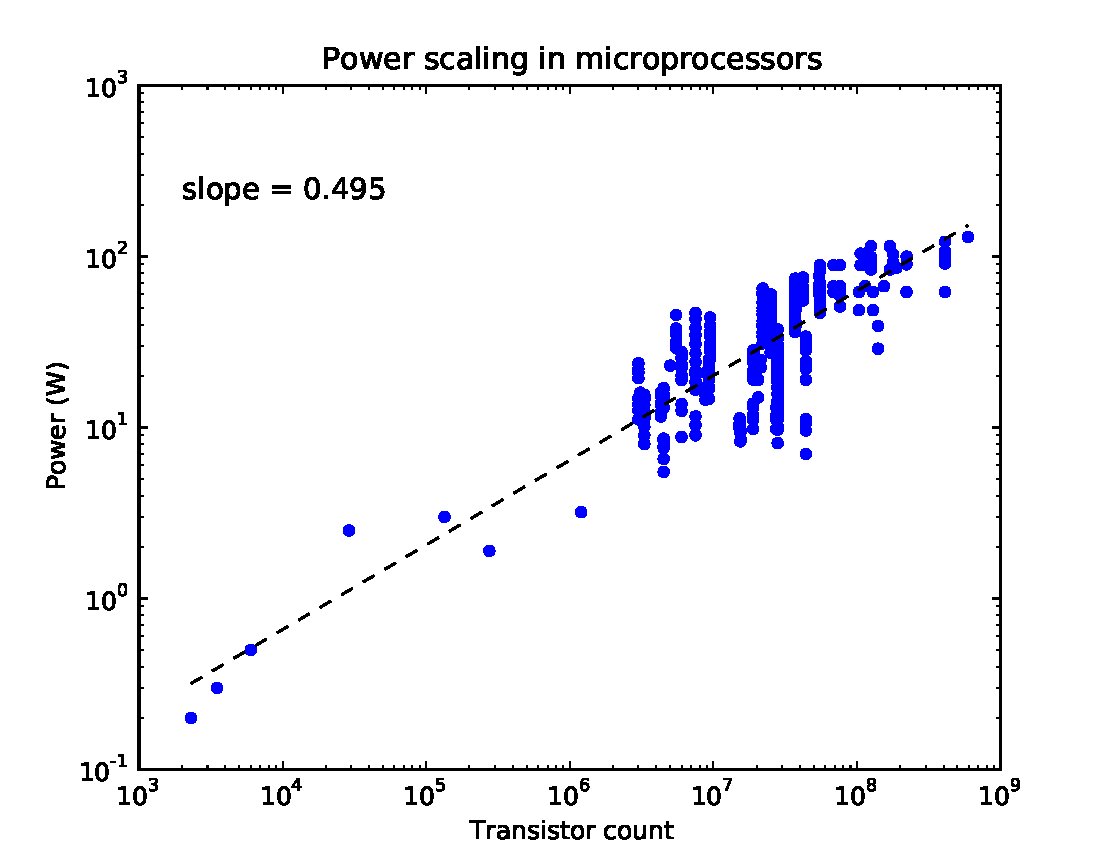
\includegraphics[height=70mm]{Figures/power_scaling.pdf}
\caption{}
\label{fig:power}
\end{figure}

\begin{figure}[!h]
\centering
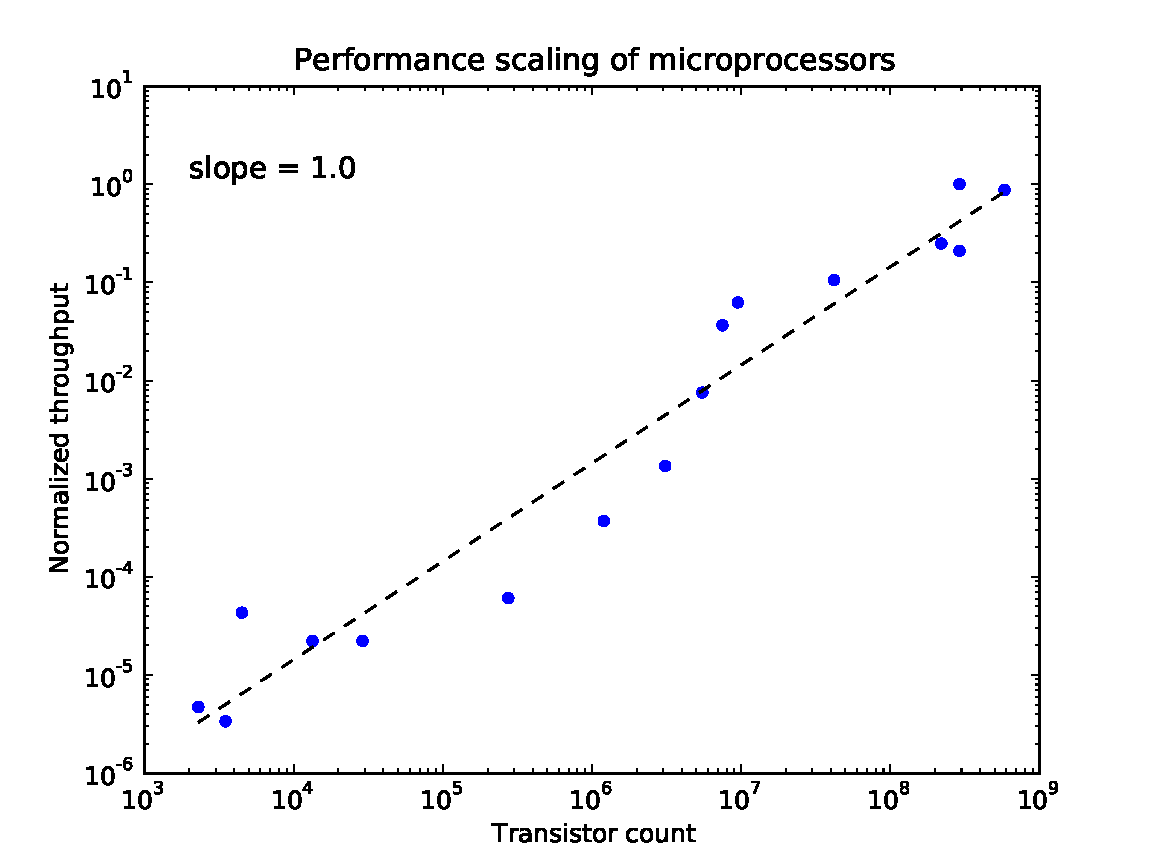
\includegraphics[height=70mm]{Figures/throughput_scaling.pdf}
\caption{}
\label{fig:throughput}
\end{figure}

Our model provides a simple theoretical explanation for the scaling of power
and performance in computers over 40 years of microprocessor technology
improvements.  The excellent agreement between the theoretical optimal and
experimental data suggests that through successive generations of
trial-and-error, innovation and optimization, engineered designs are highly
successful, approaching the theoretical limit predicted by the model.

\section{Discussion: Implications for Evolutionary Transitions}
\label{sec:discussion}

Scaling analyses provide a framework for identifying invariants and understanding constraints on both biological and computational systems over enormous size ranges. Simultaneously minimizing energy dissipation and delivery time in both the network and the nodes, predicts scaling relationships in organisms and computer chips. This broad framework also highlights similarities and differences between biological networks that deliver energy and computational networks that deliver information. 

From the similarities between biological and computational network scaling we can make predictions about the trajectory of computing based on biological changes over evolutionary time. For this we turn to work by Delong et al who demonstrate that metabolic scaling slopes and intercepts change at the evolutionary transitions: prokaryote (bacteria) metabolism is superlinear with size, unicellular protist metabolism is linear, and multicellular animal metabolism is sublinear, converging toward the canonical $3/4$ exponent. They hypothesize that these shifts arise from organisms overcoming a series of constraints, and then facing new constraints, as they increase in size.

Larger bacteria increase metabolism as additional genes allow increased use of metabolic substrates, but eventually the cell surface area limits metabolic processing. Unicellular protists internalize the metabolic machinery into respiratory organelles (i.e., mitochondria that turn oxygen into ATP). The number of mitochondria increases linearly with cell size until internal transport constraints limit the rate of metabolic processing. Multi-cellular animals develop internal networks that speed the delivery of metabolites, subject to sublinear network scaling effects. Delong et al highlight the fundamental importance of both time and energy both in the network (ie minimizing time to deliver metabolites) and in the nodes (maximizing the capacity of nodes). %They also note significant decreases in energetic efficiency at each evolutionary transition when absolute measures of time and energy increase.
The explanations that they hypothesize are directly relevant to understanding how energy-time minimization affects the ongoing evolution of computer hardware.

1.     Evolution of single core chips: The chip scaling we describe above shows how time and energy dissipation have decreased while performance increased as larger numbers of shrinking transistors have been packed onto each chip. During this period, similar to bacterial evolution that incorporates new genes to exploit new metabolic niches, technological innovations have emerged, for example, new materials, switching methods, etching processes and cooling technologies have pushed physical boundaries, allowing transistors to shrink and more of them to be packed onto each chip. Like bacteria, these innovations have optimized physical constraints, but ultimately a maximum is reached. There are no elephant-sized bacteria and there will be no silicon based single core chips with quadrillions (?) of transistors.

2.  Chips have also mimicked the linear relationship between performance and size (Figure XXX) seen in protists. Unicellular protists show linear increases in metabolic rate with size as more energy processing nodes  (mitochondria) are packed into larger cells. However, like protists, this regime will also end due to physical constraints. It is evident from the analysis above that the internal transport network already constrains the processing speed of the system (i.e., $T_{net}$ constrains $T_{sys}$). Further, the requirement to dissipate heat over a fixed surface area constrains both cells and chips. 

3. Computer chips have begun the transition to multi-core, resembling the biological transition to multicellularity. Our unified scaling framework suggests future scenarios for multicore chips. As the era of transistor minimization draws to a close, adding more transistors will require increased area, and therefore networks that span a larger area. Similarly to multicellular organisms, we expect that as the number of cores grows, an increasing fraction of chip power will be devoted to ever larger networks (Network-on-Chip, NoC) connecting more cores. Larger networks will require more power to drive them, and it will take more time to traverse them, ultimately making time-energy minimization increasingly difficult as chips increase in size. Thus we predict that networks will increasingly dominate on-chip power budgets, and the most important advances in chip design will be in increasing network efficiency, for example optical networks.
  
  
The differences between scaling of energy delivery biology and information delivery in computation also play an important role in evolutionary transitions. In particular, on-chip computer networks have two advantages not available to biological networks. First, technological advances have decreased ``process'' size by orders of magnitude over the last several decades, resulting in ever smaller transistors and wires that reduce both energy and delay in the nodes, as well as allowing the dramatic increase in the number of transistors and wires in a given area. This reduction in process size will end as physical limits are reached (although the miniaturization is predicted to continue for several more generations CITATIONS). Second, the locality of network traffic, characterized by the Rent's exponent and $D_w$, reduces long distance communication over computer networks. As shown above, this wire scaling results in lower $E_{net}$ and a smaller wire footprint as $N$ increases on single core chips. This advantage will likely continue for multi-core chips where communication, and therefore network bandwidth, footprint and energy consumption of NOCs can be reduced by keeping communication primarily local (maybe cite george here?). Communication locality has the potential to result in a more favorable scaling in multi-core computation than is achievable in multi-cellular biology.

Scaling on computer chips and other systems in which networks deliver information rather than energy also lend insights into another important biological evolutionary transition, the transition to social animal societies. Delong et al does not address scaling relationships in animal societies. However, sociality is an important evolutionary transition, reflected in the ecological dominance of humans and ants, two social species whose networked systems exchange energy and information. These social species have captured extraordinary fractions of the available energy on earth (citations�40\% globally for humans, 50\% of biomass energy in the amazon by ants) and dispersed over vast territories. Recent evidence suggests that ant colonies and human societies follow similar scaling relationships as individual organisms (citations). In social animal systems and networked computer systems, networks are at least partially decentralized, for example traffic flow in cities (CITE mosessamaniego) and communication patterns in ants (CITE Noa). Understanding how communication locality has emerged in computation may lend insights into one of the important benefits in the transition to sociality in biology: animal societies have released the constraint of the centralized distribution network by evolving systems for decentralized and modular communication.


?  PULL other TEXT from BEYOND Biology. 



%5.     The strong similarity in the scaling of computational and biological systems results from the fundamental dependence of both systems of the number of nodes (transistors in computation and �the number of membrane-bound respiratory complexes� that synthesize ATP from oxygen) and the geometric constraints on transport distances. 



\section{Conclusion}

Our analysis provides a unifying explanation for the origin of scaling laws in
biology and computing. Despite obvious differences in form and function, the
scaling of organisms and computers is governed by the same simple principle.
By minimizing energy dissipation and the time to deliver resources, whether through natural selection or
engineering, existing designs manage the trade-off between cost and
performance, leading to general scaling patterns observed over several orders
of magnitude in size.  Moreover, power laws as a function of size are not
unique to organisms and computers but are widely observed across a large
variety of complex systems in nature, society and technology.  The scaling of
white and grey matter in the brain \cite{zhang00}, of energy use and GDP in
countries \cite{brown11}, and the pace of life and population in cities
\cite{bettencourt07} are additional examples where a unifying explanation is
still lacking.  Because cost and performance, i.e., energy and time, impose
universal constraints, we suggest that a common design principle governs the
scaling of complex systems that process energy, materials and information.

Engineering ingenuity rather than evolution by natural selection has created increasingly fast and powerful computers through a series of innovations, including integrated circuits, innovations in materials and other technological tricks, synchronizing clock trees, multi-core chips and networked and distributed computation. Technological evolution is undergoing another major evolutionary transition as distributed computing changes the metabolic landscape of technology and its interaction with the environment. As computers become more embedded in physical devices, physical proximity and energy concerns for low-power devices may drive computational scaling to more closely resemble biological scaling. In computation dramatic changes have emerged over the last 35 years, but their trajectories mimic the biological transitions that took billions of years to evolve simple unicellular bacteria into the largest and most powerful animals and societies on earth.



%By unifying time and energy into a single model, the model accounts for the wide variation in size of organisms and computers, e.g., mouse to elephant and arm to multe-core.  
  
  

\section{Additional possible Discussion points. Which ones are worth keeping, and where?}

\begin{itemize} 


  
\item 
 This paragraph from before needs to be reworked here or skipped. I'm not sure if it still applies:
 
The model predicts that, for the optimal network design (i.e., $D_l=3$  and
$D_r=2$), the system's energy-time product is scales with $l_0$ and $N$.
%Since size increases with $N$, this suggests that the energy-time product is
%independent of body mass.
This result has important implications for the
energetic basis of fitness.  Some have proposed that biological fitness
maximizes metabolic power (energy/time) \cite{lotka56, odum71}, whereas others
have proposed that it minimizes biological times (e.g., generation times, which
is equivalent to maximizing vital rates) \cite{lindstedt81, sibly91}. The
invariance of the energy-time product is consistent with the fact that fitness
of organisms is largely independent of body mass.  Organisms of all sizes, from
small, fast, low-power microbes to large, slow, powerful mammals, coexist and,
therefore, are likely nearly equally fit.  This implies a direct trade-off
between maximizing metabolic power and minimizing generation times that holds
over the many orders of magnitude variation in body mass.  The energy-time
product reflects powerful geometric, physical and biological constraints on the
evolution of organism designs.


\item If we're gonna say this, we have to actually do it. I'm inclined to skip it.

 Our framework gives a theoretical explanation for well-known empirical patterns in computer
  architecture.We provide an explanation for Koomey's Law (p. 13). These results also provide an explanation for Koomey's Law, which states
roughly: ``The number of computations per joule of energy dissipated has been
doubling approximately every 1.57 years." This follows directly from minimizing
the energy time product and Moore's Law, the empirical observation that the
number of transistors ($N$) doubles every 2 years. NEED a figure that combines
data from Fig 2 and Fig 3 to show this?



%\item Nature dealt with network design constraints by slowing metabolism as
%  animal size increases.  Computer architecture, at least until recently,
%  focused on increase clock speeds by minimizing component size and incresing
%  energy per chip.  Also, using the third dimension to accommodate more wires, 

%\item Computer transitons: transistors; transistors to integrated circuits;
%  single core to multi-core; desk tops to data centers.  Multicore is an
%  evolutionary transition.  IBM currently making 10 nm chips which are the
%  limit for silicon.  IBM recently announced a 7 nm transistor (more than 1000
%  times smaller than the diameter of a red blood cell) and only three times
%  larger than a strand of DNS, using silicon germanium targeting a 50\% power
%  improvement.  NYT July 9, 2015.  Then going to carbon nanofibers. 
  
\end{itemize}



\section{Appendix A: Details of Scaling in Organisms}
\label{sec:AppendixOrg}

In this section we give a detailed analysis of the derivation of the scaling of
the total network resistance discussed in Sec.~\ref{sec:organisms}. Recall
that $D_l = 3$ for $3$ dimensional organisms and that $\lambda^{-H}=N^{-1}$.
Using these values and simplifying, equation~\ref{eq:resistance} is
transformed. 

\begin{equation}
 R = \frac{8 \mu l_0}{\pi r_0^4} N^{-1} \sum_{i=0}^H \lambda^{i(\frac{4}{3} -\frac{4}{D_r})}
\end{equation}

Let the summand $S = \sum_{i=0}^H \lambda^{i(\frac{4}{3} -\frac{4}{D_r})}$. $R \propto
N^{-1} S$. How $S$ scales with $N$ is dependent on the exponent $\frac{4}{3} -
\frac{4}{D_r}$, and reduces to four different cases:

\begin{caseof}

    \case{$D_r=3$}{In this case the exponent is equal to 0, and the $S = H+1
    \propto \log (N)$, and $R\propto \frac{\log(N)}{N}$, because $\log(N)$ in
  this case grows much more slowly than $N$, it is reasonable to conclude that
$R\propto N^{-1}$}

    \case{$D_r < 3$}{Here (and in subsequent cases) we can use the geometric series to
      calculate the exact value of $S$. In particular 

      \begin{align*}
        S &= \frac{(1-\lambda^{(\frac{4}{3}
    -\frac{4}{D_r})(H+1)})}{1-\lambda^{\frac{4}{3} -\frac{4}{D_r}}} \\ 
        &= \frac{1-\left(\lambda^{H}\right)^{(\frac{4}{3}-\frac{4}{D_r})}
      \lambda^{(\frac{4}{3} - \frac{4}{D_r}))}}{1-\lambda^{\frac{4}{3}
      -\frac{4}{D_r}}} \\
        &= \frac{1-N^{(\frac{4}{3}-\frac{4}{D_r})}
      \lambda^{(\frac{4}{3} - \frac{4}{D_r}))}}{1-\lambda^{\frac{4}{3}
           -\frac{4}{D_r}}}
      \end{align*}

      If we let $c = \lambda^{(\frac{4}{3} -\frac{4}{D_r})}$ we see that

      \begin{equation}
        S = \frac{1-c N^{(\frac{4}{3}-\frac{4}{D_r})}}{1-c}
      \end{equation}

      Because $\frac{4}{3} - \frac{4}{D_r} < 0$ is negative in this case
      and $N$ is large in practice, $c N^{(\frac{4}{3} -\frac{4}{D_r})}$ is
      small, and $S$ is proportional to a constant ($S \approx
    \frac{1}{1-c}$). This implies that $R \propto N^{-1}$.}

    \case{$3 < D_r < 12 $}{In this case the exponent in $S$ is positive,
      meaning that $S$ scales directly with $N$. Note that $c>1$ in this case
      and we can write 
      \begin{equation}
        S = \frac{c N^{(\frac{4}{3}-\frac{4}{D_r})}-1}{c-1}
      \end{equation}

      \noindent This means that $S \propto N^{(\frac{4}{3} - \frac{4}{D_r})}$.
      This implies that $R \propto N^{-1} S \propto N^{(\frac{1}{3}
      -\frac{4}{D_r})}$. This means that resistance still scales inversely with
      size, but at a faster rate than if $D_r \leq 3$.}

   \case{$D_r \geq 12$}{This final case is analogous to the one above, except
   that now resistance scales positively with $N$, implying that the energy in
 the network would scale positively with $N$. This is likely a non-physical
 possibility, but we include it here for completeness.}

\end{caseof}

\section{Appendix B: Details of Scaling in Electronics}
\label{sec:AppendixChips}

In this section we give a detailed analysis of the derivation of the scaling of
the network capacitance and network latency discussed in
Sec.~\ref{sec:computers}.

\subsection{Capacitance}

Recall that $D_l = 2$ for $2$ dimensional computer
chips and that $\lambda^{-H}=N^{-1}$. We can then calculate capacitance as:

\begin{equation}
  C \propto  N^{(1- \frac{1}{D_l}} \sum_{i=0}^H \lambda^{i \left( 
\frac{1}{D_l} + \frac{1}{D_w} -1 \right)}
\end{equation}

Similar to how we handled organsims we are interested in whether the exponent
$\frac{1}{D_l} + \frac{1}{D_w} -1$ is positive or negative.

Let the summand $S = \sum_{i=0}^H \lambda^{i(\frac{1}{D_l} +
\frac{1}{D_w}-1)}$. $C \propto
N^{1-\frac{1}{D_l}} S$. 

\begin{caseof}

  \case{$D_r=\frac{D_l}{D_l-1}$}{In this case the exponent is equal to 0, and the $S = H+1
    \propto \log (N)$, and $C\propto \log(N) N^{1-\frac{1}{D_l}}$, because $\log(N)$ in
    this case grows much more slowly than $N^{1-\frac{1}{D_l}}$ and we know
    $D_l=2$ for 2 dimensional chips, it is reasonable to conclude that
  $C\propto N^{\frac{1}{2}}$}

  \case{$D_r > \frac{D_l}{D_l-1}$}{Here (and in subsequent cases) we can use
    the geometric series to calculate the exact value of $S$, using a similar
  approach to~\ref{Appendix:Org}. In this case the exponent is negative and $S$
is a small constant, leaving $C \propto N^{\frac{1}{2}}$}

\case{$D_r < \frac{D_l}{D_l-1} $}{In this case the exponent in $S$ is positive,
      meaning that $S$ scales directly with $N$. Now the summand contributes an
    $N^{\frac{1}{D_l}+\frac{1}{D_w} -1}$ and $C \propto N^{\frac{1}{D_w}}$.}

\end{caseof}

\subsection{Network Delay}

Recall that we wish to determine the network latency $L$ which is defined as:

\begin{equation}
  T_{net} \propto \max_{i} L_i
\end{equation}

\noindent with

\begin{equation}
  L_i \propto RC = \frac{\rho \epsilon li^2}{r_i^2} = \frac{\rho \epsilon
  l_0^2}{r_0^2} \lambda^{i\left(\frac{2}{D_l} - \frac{2}{D_r}\right)}
\end{equation}

\noindent $L_i$ will scale differently depending on the relative values of
$D_r$ and $D_l$. 

\begin{caseof}

  \case{$D_r>D_l$}{In this case the fraction in the exponent is greater than 0
  and the latency will be highest when $i=H$, resulting in $L \propto
N^{\frac{2}{D_l} - \frac{2}{D_r}}$. }
  
  \case{$D_r <  D_l$}{In this case the exponent is negative and the highest
  latency occurs at the bottom of the network $i=0$, leaving $L\propto
\frac{l_0^2}{r_0^2} \propto N^0$}

  \case{$D_r = D_l$}{In this case the exponent is 0 and there is equal latency
  at all levels and $L \propto N^0$.}
\end{caseof}



\bibliography{references}
\bibliographystyle{abbrv}

\newpage

\section*{Figure legends}
\paragraph{Figure 1:} Log-log plot of power consumption as a function 
of transistor count for 523 computer microprocessors from different 
vendors and technological generations.  The linear regression slope is 
$0.495$ with correlation coefficient of $0.81$. A regression that 
removes the first seven data points and focuses on the main cloud of 
more modern chips produces a slope of $0.487$.

\paragraph{Figure 2:} Log-log plot of normalized throughput as a 
function of transistor count for 16 Intel microprocessors from 
different technological generations.  The linear regression slope is 
1.0 with correlation coefficient of 0.97.

\end{document}



